\newcommand\drawrectangle[6]{
  \draw[#5, thick, fill=#5!30, opacity=.8] (#1, #2) rectangle ++(#3, #4);%
  \fill[#5] (#1, #2) circle (.2cm);
  \node[#5] at ({#1 + #3/2}, {#2 + #4/2}) {#6};
}

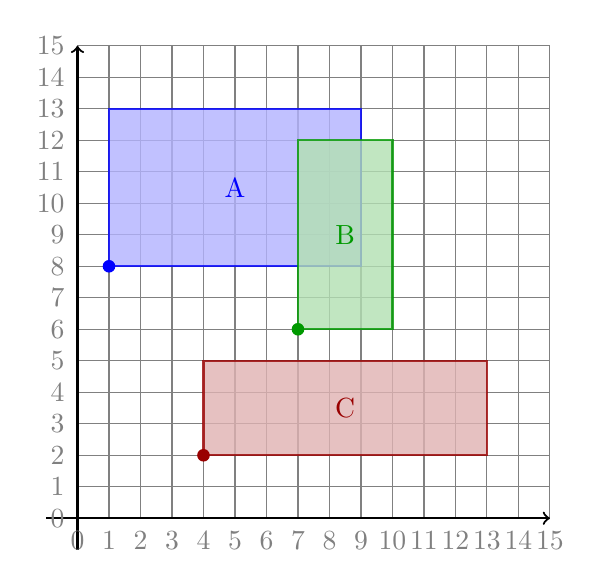
\begin{tikzpicture}[scale=.4]

  \def\gridsize{15}
  \draw[gray] (0, 0) grid (\gridsize, \gridsize);
  \draw[thick,->] (-1, 0) -- (\gridsize, 0);
  \draw[thick,->] (0, -1) -- (0, \gridsize);

  \drawrectangle{1}{8}{8}{5}{blue}{A}
  \drawrectangle{7}{6}{3}{6}{green!60!black}{B}
  \drawrectangle{4}{2}{9}{3}{red!60!black}{C}

  \foreach\i in {0,...,\gridsize} {
      \node[gray, anchor=north] at (\i, -.1) {\i};
      \node[gray, anchor=east] at (-.1, \i) {\i};
  }

\end{tikzpicture}

